% ------------------------------------------------------------------------------
% TYPO3 CMS 7.6 - What's New (English Version)
%
% @author	Patrick Lobacher <patrick@lobacher.de> and Michael Schams <schams.net>
% @license	Creative Commons BY-NC-SA 3.0
% @link		http://typo3.org/download/release-notes/whats-new/
% @language	English
% ------------------------------------------------------------------------------
% LTXE-CHAPTER-UID:		d71b4b88-f79b2343-d2b356bf-452cef81
% LTXE-CHAPTER-NAME:	Backend User Interface
% ------------------------------------------------------------------------------

\section{Interfaccia utente Backend}
\begin{frame}[fragile]
	\frametitle{Interfaccia utente Backend}

	\begin{center}\huge{Capitolo 1:}\end{center}
	\begin{center}\huge{\color{typo3darkgrey}\textbf{Interfaccia utente Backend}}\end{center}

\end{frame}

% ------------------------------------------------------------------------------
% LTXE-SLIDE-START
% LTXE-SLIDE-UID:		e1b76ec4-6cbb40b6-bca20a01-f9cb76a8
% LTXE-SLIDE-ORIGIN:	d8599a04-11b4fa8c-9be5812a-715820e1 English
% LTXE-SLIDE-ORIGIN:	ef1d6d8c-0db67396-dedb5814-1767169f German
% LTXE-SLIDE-TITLE:		Rework workspace notification settings (1)
% LTXE-SLIDE-REFERENCE:	Feature-35245-ReworkWorkspaceNotificationSettings.rst
% ------------------------------------------------------------------------------
\begin{frame}[fragile]
	\frametitle{Interfaccia utente Backend}
	\framesubtitle{Impostazioni di notifica del Workspaces (1)}

	Le modalità e il comportamento delle impostazioni di notifica sono state snellite\newline
	\smaller(una procedura guidata consente di aggiornare le impostazioni)\normalsize

	\begin{figure}
		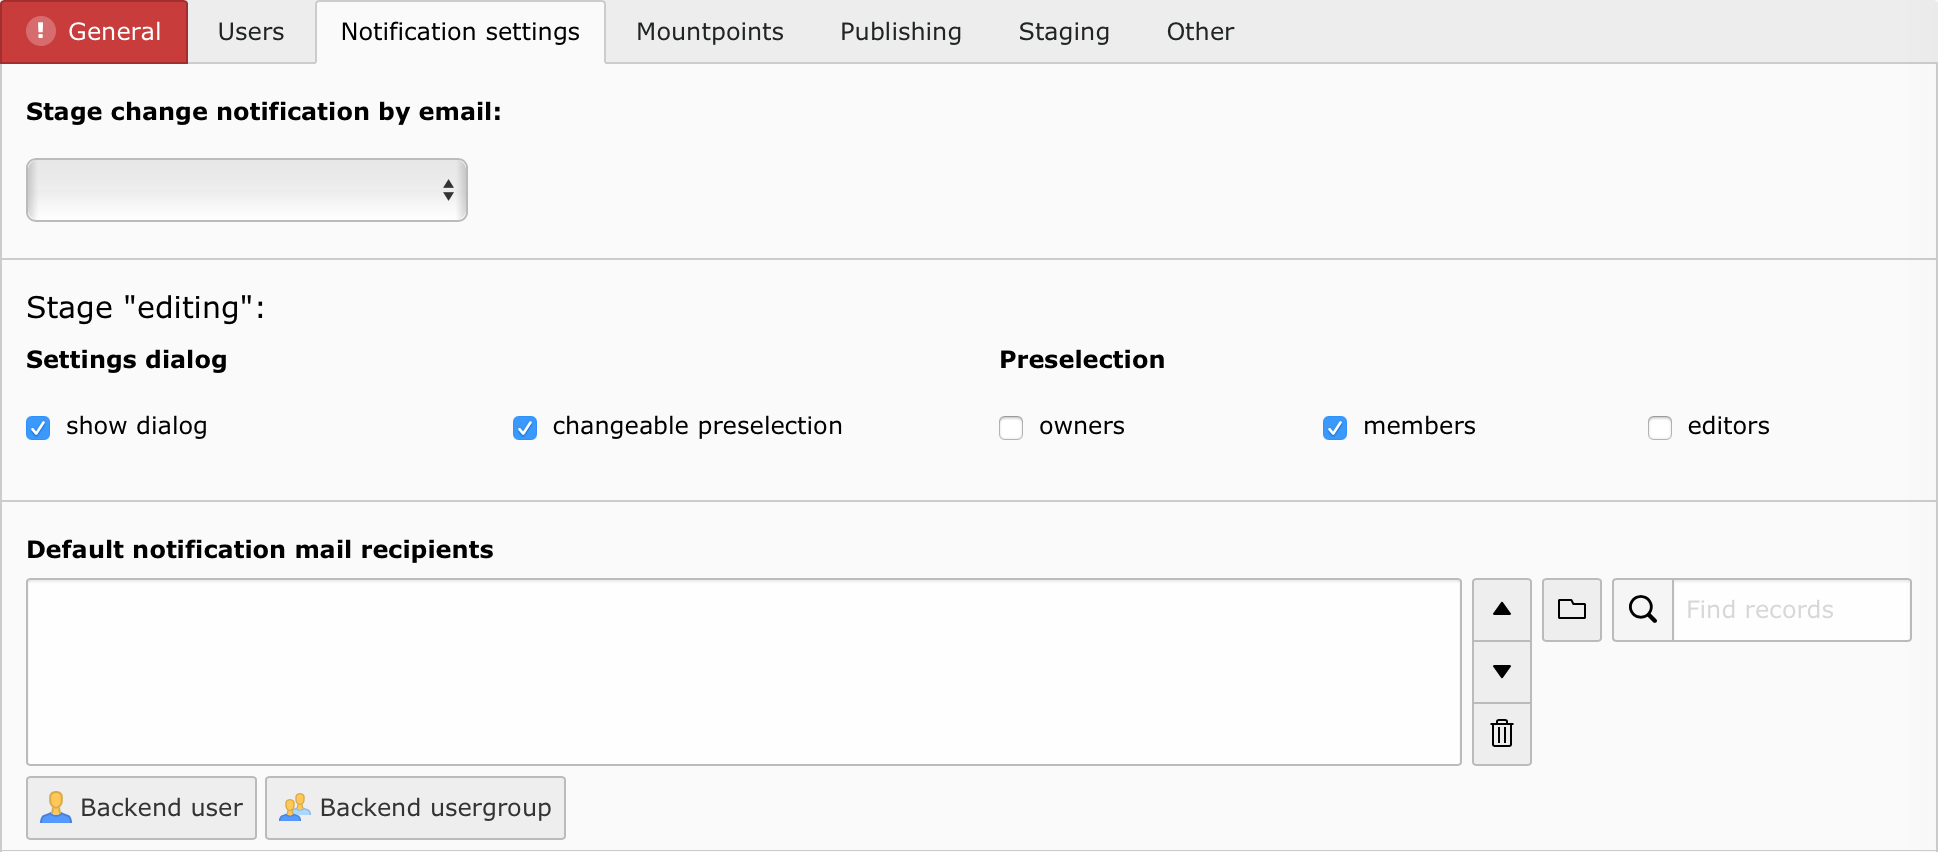
\includegraphics[width=0.94\linewidth]{BackendUserInterface/35245a.png}
	\end{figure}

\end{frame}

% ------------------------------------------------------------------------------
% LTXE-SLIDE-START
% LTXE-SLIDE-UID:		691cd805-0bcd6433-7228a8c2-88b76e93
% LTXE-SLIDE-ORIGIN:	04855567-dac16e24-f5274c64-f1d49c36 English
% LTXE-SLIDE-ORIGIN:	1db1430d-4db24c16-2bf357bb-5f5c85db German
% LTXE-SLIDE-TITLE:		Rework workspace notification settings (2)
% LTXE-SLIDE-REFERENCE:	Feature-35245-ReworkWorkspaceNotificationSettings.rst
% ------------------------------------------------------------------------------
\begin{frame}[fragile]
	\frametitle{Interfaccia utente Backend}
	\framesubtitle{Impostazioni di notifica del Workspaces (2)}

	Lo stage "\textbf{publishing execute}" riceve le opzioni di configurazione

	\begin{figure}
		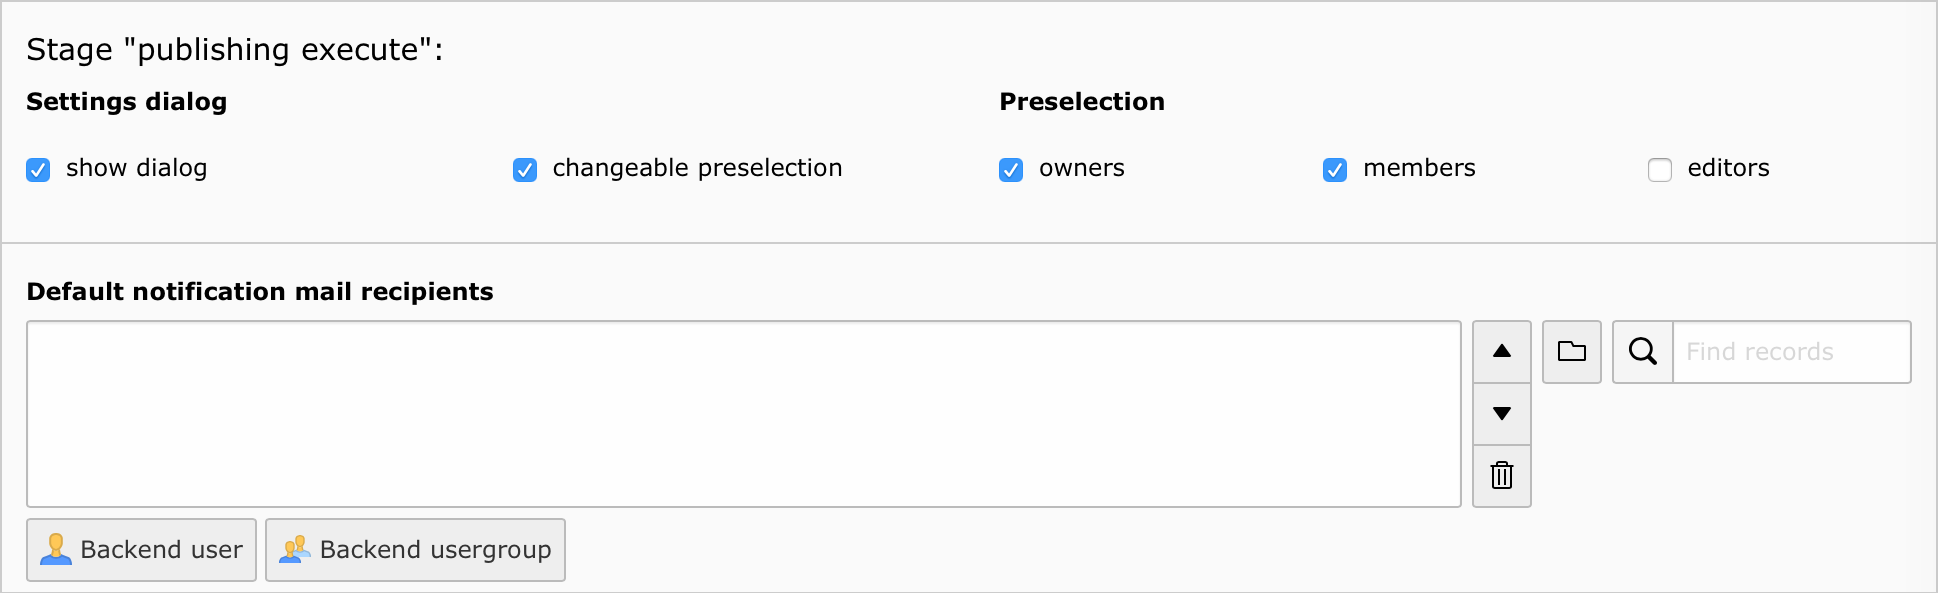
\includegraphics[width=0.94\linewidth]{BackendUserInterface/35245b.png}
	\end{figure}

\end{frame}

% ------------------------------------------------------------------------------
% LTXE-SLIDE-START
% LTXE-SLIDE-UID:		ba10fe96-822cca92-7a29e38d-953f4a39
% LTXE-SLIDE-ORIGIN:	fd6d762a-b268caf0-cb6f9195-f553e035 English
% LTXE-SLIDE-ORIGIN:	80fbd7db-2c4c98db-06e09bb9-ef0a5112 German
% LTXE-SLIDE-TITLE:		Add basic file search in element browser
% LTXE-SLIDE-REFERENCE:	Feature-69120-AddBasicFileSearchInElementBrowser.rst
% ------------------------------------------------------------------------------
\begin{frame}[fragile]
	\frametitle{Interfaccia utente Backend}
	\framesubtitle{Funzione di ricerca nell'Element Browser}

	La ricerca file è stata aggiunta all'Element Browser di TYPO3 (funziona ricorsivamente)

	\begin{figure}
		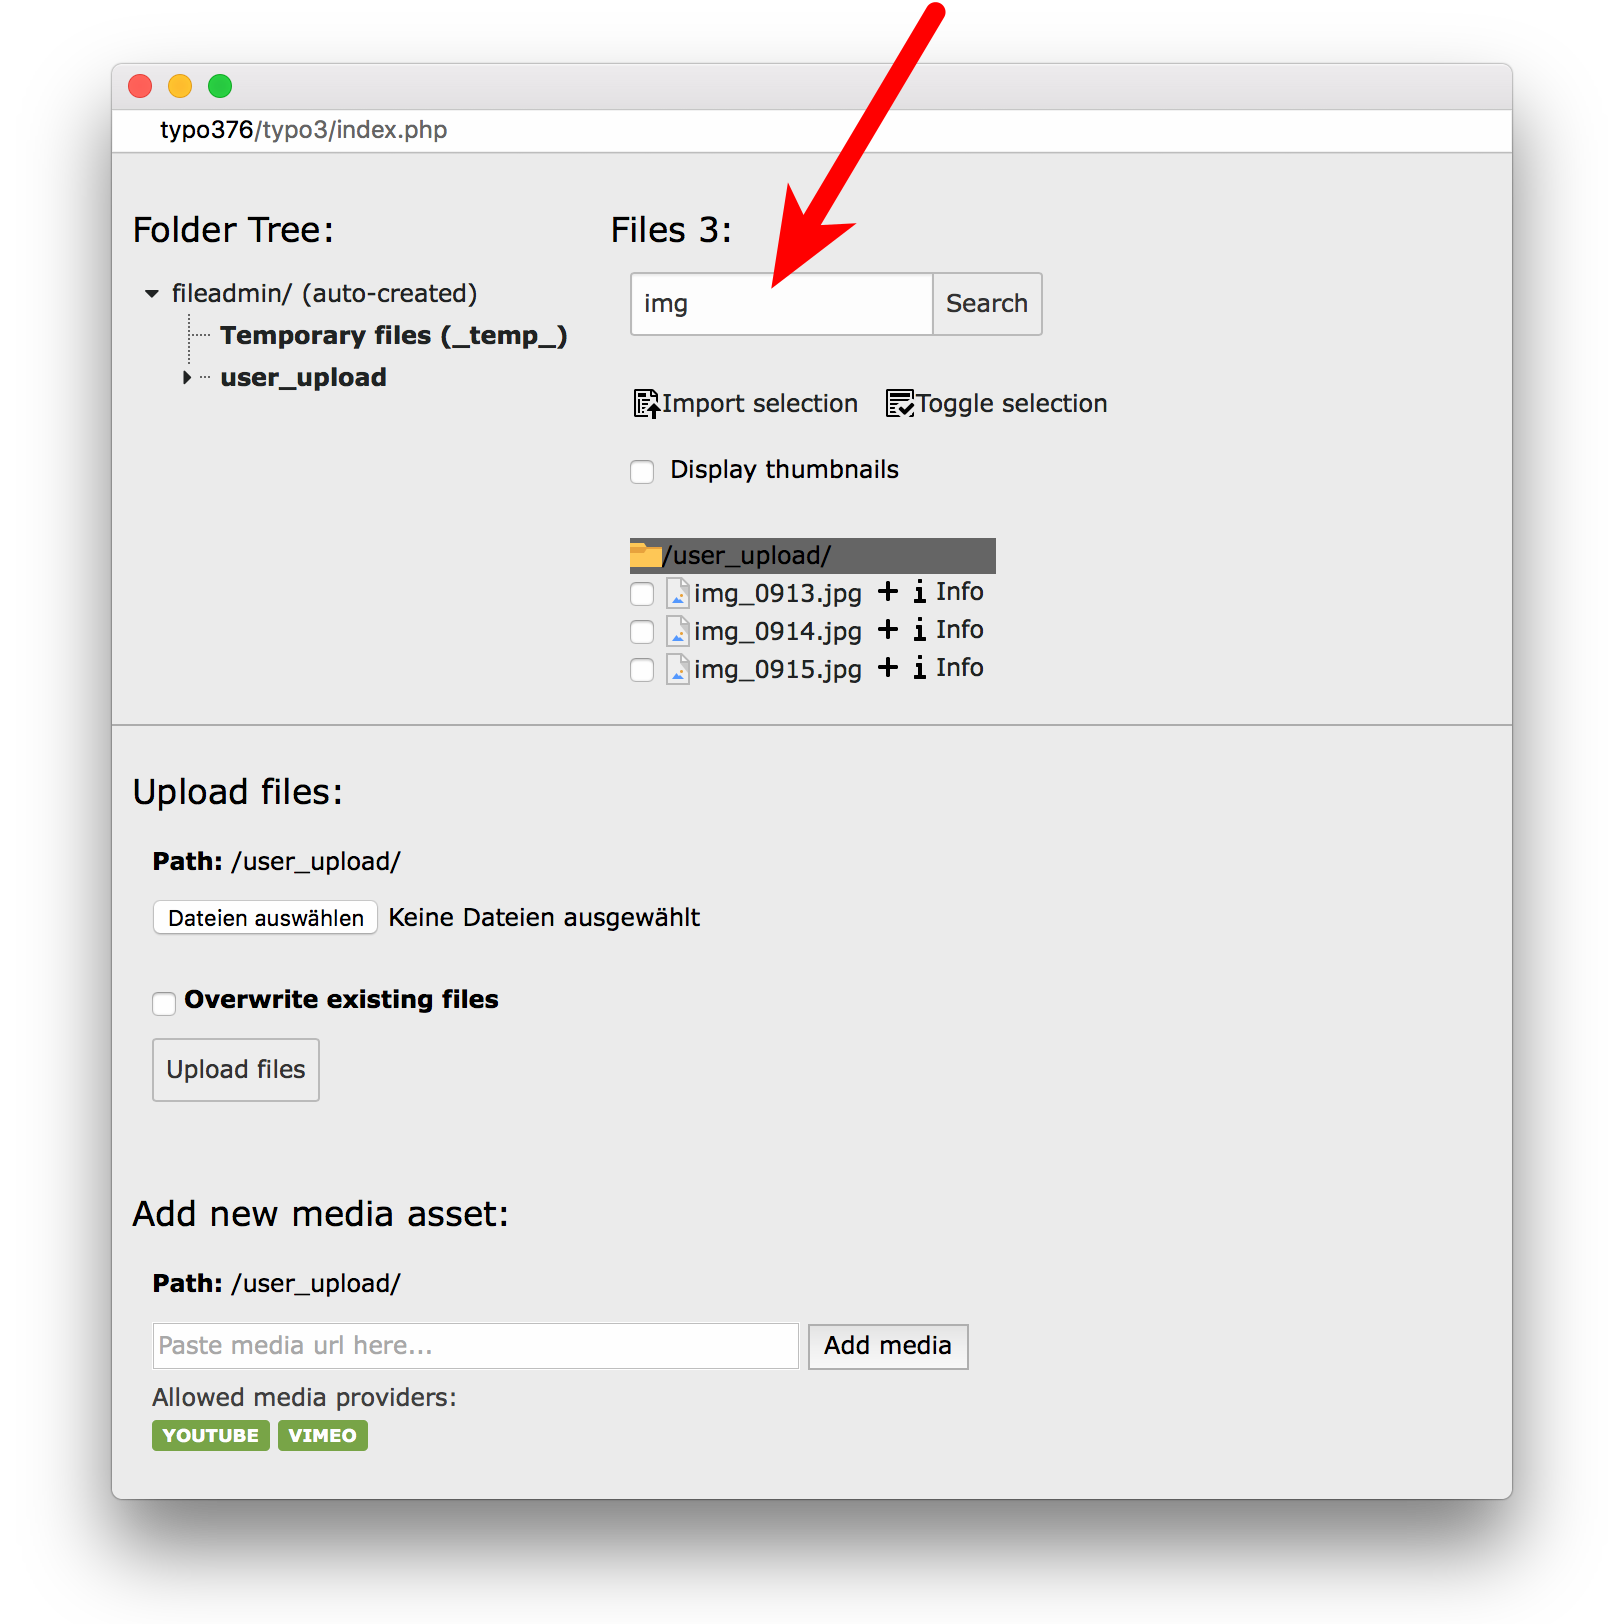
\includegraphics[width=0.4\linewidth]{BackendUserInterface/69120.png}
	\end{figure}

\end{frame}

% ------------------------------------------------------------------------------
